\chapter{Propuesta de Sistema Central de Autenticación}\label{chapter:proposal}
En el siguiente capítulo se presenta una solución al problema principal de la tesis. Se presenta la hipótesis del problema y los requisitos del software. También se explica por capas las varias etapas que el software debe tener: bases de datos, ingestión de datos, capa de autenticación, clientes y usuarios. En cada una de estas se analizan los problemas que debe resolver y se estudia cómo deben ser resueltos.
\section{Hipótesis}
La Universidad de la Habana cuenta con varios sistemas en la red donde se utiliza el método tradicional de usuario/contraseña como mecanismo de seguridad para acceder a diversas aplicaciones, este proceso de autenticación se hace muy complejo al tener que acceder a cada uno de ellos de forma independiente. Con cada servicio nuevo se debe crear un sistema de autenticación que garantice la seguridad de sus datos y se debe hospedar la información de los usuarios repetidas veces, lo cual utiliza una mayor cantidad de recursos y es más propenso a fallas.

Para eliminar estas dificultades se diseña un sistema central de autenticación que se basa en el método Inicio de Sesión Único. Esta propuesta tiene como propósito un aumento en la productividad, ofrecer mayor facilidad de acceso a los recursos, funciones de autenticación a través de una única plataforma, una administración sencilla de credenciales y sobre todo garantizar un aumento de la seguridad. Mediante este servicio el usuario podrá registrarse en el sistema una sola vez, con lo cual podrá acceder a todos los recursos sin tener que volver a autenticarse.


\subsection{Requisitos del Software:} \label{software-req}
\begin{itemize}
	\item Unificar las distintas fuentes de datos.
	\item Que el usuario inicie sesión y, hasta que cierre sesión, sea capaz de realizar operaciones sin tener que volver a introducir credenciales. 
	\item El servicio ofrecido al cliente debe permitir que el usuario extienda la sesión una vez pasado el tiempo de expiración de la misma sin tener que volver a introducir credenciales. 
	\item Reconocer la identidad de los usuarios durante el proceso de autenticación para garantizar un adecuado control de acceso a los recursos del sistema.
	\item Proteger los recursos del sistema, permitiendo que estos sean solamente usados por aquellos usuarios a los que se les ha concedido autorización.
	\item Que el usuario inicie sesión con dos únicos campos: nombre de usuario y contraseña. Este requisito será suficiente para garantizar la interoperabilidad del sistema, que debe ser capaz de generar un objeto encriptado con toda la información relativa a dicho usuario y viajar por la red de comunicaciones entre las distintas entidades. 
	\item  La respuesta obtenida al iniciar sesión de forma exitosa debe ser un objeto que le dé portabilidad y reusabilidad al software.
	\item En caso de obtener un inicio de sesión erróneo, retornar un error.
	\item Garantizar el control de errores y excepciones.
	\item La evaluación de permisos de acceso.
\end{itemize}

El software consta de varias etapas:

\begin{figure}[H]
	\centering
	\hspace*{-0.5in}
	\includegraphics[width=1.2\linewidth]{"Graphics/Diagrama Tesis"}
	\caption{Etapas de implementación del software}
	\label{fig:diagrama-tesis}
\end{figure}

\section{Bases de Datos} \label{db-layer}

%que es
Actualmente los estudiantes de toda la Universidad de La Habana al matricularse se inscriben en Secretaría en el Sistema de Gestión de la Nueva Universidad (SIGENU). En este sistema se almacenan todos los datos de los alumnos: datos personales, proveniencia, notas, grados.

Por otra parte, los datos de los profesores y del resto de los trabajadores de la universidad son guardados en bases de datos de ASSETS, software contratado. Cada unidad presupuestada de la universidad tiene su propio ASSET donde se almacena los datos de recursos humanos y del inventario.

%problema
El Nodo Central es el responsable de todas las comunicaciones de la Universidad de La Habana. Presta servicios a todas las facultades, desde las que se encuentran en la Colina, hasta facultades externas como Economía, el Jardín Botánico y la Quinta de los Molinos. Cada facultad tiene su sistema independiente, que responde a sus necesidades, donde gestiona a todo su personal. 

La información es almacenada en varias bases de datos, lo cual hace difícil la gestión de todos los usuarios de la Universidad. Crear un sistema único al cual todas las facultades pudieran acceder de forma remota simplificaría el trabajo, no solo a los programadores, sino también a los usuarios. Por ejemplo, cada estudiante podría matricularse en su propia facultad y se evitarían las aglomeraciones y la confusión creada cada año. 

Sin embrago, sería complicado cambiar el software utilizado por toda la institución. Como se mencionó anteriormente, algunas facultades se encuentran alejadas de La Colina, lo cual dificulta la comunicación y la instalación de nuevos sistemas. También se debe tener en cuenta que la experiencia del usuario sería diferente con un nuevo software. El personal de la universidad es de variadas edades, por lo que podría ser complejo la adaptación a una nueva interfaz.

% propuesta
Por lo tanto, en el presente trabajo se ha decidido no cambiar los sistemas. La unificación de las bases de datos de usuario de toda la Universidad de La Habana es un proceso complejo que no se encuentra en los objetivos del presente trabajo. 

\section{Ingestión de Datos} \label{data-layer}
La ingesta de datos es el proceso mediante el cual se introducen datos, de diferentes fuentes,
estructura o características dentro de otros sistemas de almacenamiento o procesamiento de
datos.  [\cite{fernandez2020aplicacion}]

Teniendo varias fuentes de datos, para garantizar una ingestión de datos exitosa, la solución debe ser capaz de leer información de distintas fuentes de datos. 

Por otra parte, el estado de un usuario puede cambiar y sus permisos de acceso pueden variar. Por ejemplo, a los estudiantes se les puede dar baja o un trabajador puede terminar su contrato y, por lo tanto, se les debe retirar sus credenciales de forma inmediata. Un estudiante después de graduarse puede pasar a ser trabajador de la institución, por lo que sus permisos de acceso deben ser cambiados. Otro caso sería cuando un estudiante o trabajador sale de licencia, deben suspenderse sus credenciales temporalmente hasta que la persona regrese. 

Se necesita que el sistema de autenticación se actualice constantemente ya que la información en las bases de datos cambia todo el tiempo.

La Universidad  se encuentra en constante cambio. Por ejemplo, en 2017 culminó el proceso de adscripción del Instituto Superior de Diseño (ISDI) a la Universidad de La Habana [\cite{isdi-historia}]. Para ello fue necesario incorporar todos los datos de los usuarios del ISDI al sistema de autenticación vigente para otorgarles las credenciales correspondientes. Por ello, el nuevo sistema debe ser capaz de admitir nuevas fuentes de datos de forma sencilla en un futuro. 

En el nodo central, la ingesta de datos se hace a través de LDAP.

% \textcolor{red}{(explicar brevemente para qué se usa LDAP en el nodo y cómo ingesta los datos)}

\section{Capa de Autenticación} \label{auth-layer}
El proceso de autenticación consiste en la verificación de la identidad de un usuario o una entidad  [\cite{teheran2014mecanismo}]. La certificación de credenciales es un área clave en la seguridad de la información. En la modernidad los usuarios necesitan acceder a muchos servicios digitales imprescindibles para su vida cotidiana. Las contraseñas basadas en caracteres alfanuméricos han sido las más comunes en todo tipo de sistemas por su fácil implementación [\cite{rodriguez2018seguridad}].

En este caso la capa de autenticación es la encargada de recibir las peticiones de los distintos clientes y verificar la identidad de un usuario a partir de la información recopilada por la ingestión de datos.

Los usuarios de la Universidad de La Habana  utilizan diariamente distintos servicios, que van desde acceder a Internet por la red WI-FI o por proxy, hasta servicios web como EVEA y correo. Cada servicio tiene su propio sistema de autenticación, lo cual causa molestias y dificultades en la interacción con las plataformas de los usuarios y complejiza el trabajo de los programadores.

Resulta engorroso crearse una cuenta en cada uno de los sistemas y autenticarse cada vez que uno acceda a un sitio nuevo. La creación de un sistema en el cual todos los usuarios de la Universidad puedan autenticarse con su correo de la institución y su contraseña facilitaría la interacción diaria con los servicios ofrecidos por el Nodo Central.


Como se ha explicado, el nuevo sistema unificará la autenticación de todos los servicios prestados por la Universidad. Para ello se utilizará el método Single Sign-On, mecanismo que permite a un usuario acceder a múltiples servicios utilizando una sola credencial. Esto significaría que si se tiene una cuenta de correo con la que se puede acceder a un sitio, no será necesario registrarse en el resto de los servicios.

El programa también debe garantizar la seguridad de las cuentas. Por ejemplo, los estudiantes utilizan las máquinas de los laboratorios y se autentican con su cuenta personal. Es común que las personas olviden cerrar sus sesiones, por lo que la cuenta debe expirar al pasar un tiempo prudencial, de lo contrario, su información puede ser utilizada por otra persona. La utilización de la autenticación basada en \textit{tokens} facilita el cierre de sesión de forma automática luego de un determinado tiempo.

Este sistema permitirá a todos sus clientes conectarse de forma segura y sencilla para que verifiquen las credenciales de sus usuarios. La universidad actualmente ofrece muchos servicios, por lo que se debe encontrar la forma óptima de migrar los clientes a la nueva forma de autenticar.


\section{Clientes} \label{client-layer}
El cliente es un programa ejecutable que participa activamente en el establecimiento de las conexiones. Envía una petición al servidor y se queda esperando por una respuesta. [\cite{lizama2016redes}]

\begin{figure}[H]
	\centering
	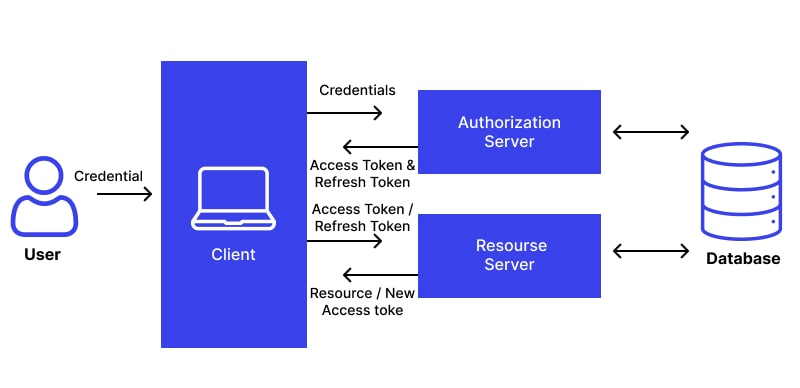
\includegraphics[width=0.9\linewidth]{Graphics/token-based-auth}
	\caption{Flujo de información desde el cliente hasta la base de datos}
	\label{fig:token-based-auth}
\end{figure}

El Nodo Central brinda infraestructura a los clientes de la Universidad vitales para el correcto funcionamiento de la institución. Entre sus responsabilidades se encuentran la gestión de correo, el acceso a Internet, las cuentas de usuarios y en el caso de los profesores gestión de cuentas de VPN. También tiene como clientes todos los servicios web de la casa de altos estudios, entre ellos el sitio oficial de la Universidad \url{https://www.uh.cu/} y los sistemas utilizados en recursos humanos y en los departamentos de contabilidad.

La creación de un sistema central de autenticación facilitaría el trabajo de los programadores que se ven obligados a crear un nuevo servicio de autenticación para cada aplicación. Sería más eficiente respecto a los recursos utilizados porque se unificarían todas las bases de datos utilizadas por cada programa para mantener los registros de sus usuarios. El tráfico de información se minimizaría ya que los usuarios solo tendrían que autenticarse una única vez para tener acceso a todos los servicios de la Universidad, por lo que se reducen las congestiones en los servidores y el tiempo de respuesta. También disminuirían las brechas de seguridad que existen y, por tanto, se minimizaría el volumen de información sensible en la red expuesta a ataques externos.

El software debe ser capaz de admitir un alto número de clientes y debe facilitar la adición de uno nuevo.

Uno de los clientes más importantes es el Entorno Virtual de Enseñanza y Aprendizaje, más conocido como EVEA, creado en 2018. El sitio es una plataforma informática encargada de orientar la comunicación pedagógica entre los universitarios que intervienen en el proceso educativo. También, tiene la misión de crear espacios o comunidades organizadas en torno al estudio. [\cite{evea-cd}] 

Este entorno virtual representó un apoyo para el sistema universitario cuando los estudiantes no podían asistir a sus facultades debido a la pandemia provocada por la Covid-19 en diciembre del 2019 [\cite{ferrer2020pandemia}]. En la primera mitad del año 2020 la cantidad de usuarios aumentó considerablemente en poco tiempo. El sistema era lento y tenía muchas fallas. Uno de los mayores retos fue lograr registrar a todos sus usuarios y que estos se pudieran autenticar. De haber existido un sistema que ya autenticara a todos los estudiantes y profesores de la universidad, los programadores habrían tenido un problema menos a la hora de modificar la plataforma para adaptarla al nuevo uso que se le daría.

\section{Usuarios} \label{user-layer}

Los usuarios de la Universidad de La Habana se encuentran en un amplio rango de edades. Se encuentran matriculados 38 678 estudiantes en cursos de pregrado, maestrías, doctorados y otros cursos. Entre los trabajadores se encuentran 600 docentes, personal de administración y servicio, economistas, entre otros. Es un grupo muy heterogéneo, lo cual se debe tener en cuenta para el desarrollo de una aplicación.

Con el uso de distintos sistemas de autenticación, los usuarios se ven obligados a tener más de una credencial lo cual crea confusión. Frecuentemente se olvidan los nombres de usuarios o contraseñas o se utilizan las mismas credenciales en varios sitios, lo cual es una mala práctica desde el punto de vista de la seguridad y es confuso y complejo para muchos. Es muy fácil olvidar las credenciales, lo cual obliga a los gestores del sistema del Nodo Central a enviar un correo no encriptado con información confidencial. Por otra parte, frecuentemente los usuarios se ven obligados a dirigirse a los especialistas por problemas con sus cuentas. 

Un nuevo sistema centralizado de autenticación beneficiaría a los usuarios ya que solo tendrían una cuenta para acceder a todas las aplicaciones. También será más fácil gestionar una sola cuenta.